\documentclass{article}

\usepackage{graphicx, xcolor}
\usepackage{amsmath, amssymb}
\usepackage{float}
\usepackage[colorlinks=true,allcolors=blue]{hyperref}

\usepackage[margin=1in]{geometry}

\def\hwtitle{Homework 7: The Bootstrap Method}
\def\hwauthor{Caden Gobat}
\def\hwdate{\today}

\usepackage{fancyhdr}
\lhead{\hwauthor}
\chead{\hwtitle}
\rhead{\hwdate}
\lfoot{\hwauthor}
\cfoot{}
\rfoot{\thepage}
\renewcommand{\footrulewidth}{0.4pt}
\pagestyle{fancy}

\author{\hwauthor}
\title{\hwtitle}
\date{\hwdate}

\begin{document}

\maketitle
\thispagestyle{fancy}

\section{Introduction}

In this assignment, we return to fitting functions to data, but this time using a more advanced technique than last week: bootstrapping. Bootstrapping and Monte Carlo methods in our case rely on the assumption that every data point and corresponding error represent their own normal distribution. When this is the case, we can ``resample'' data by randomly reassigning the value of each $y_i$ within a parameter space defined by a Gaussian centered on its original value with a width of its associated error, $\sigma_i$. Doing this for every point in the dataset many times over and fitting a function each time will give us a number of fits, which we can then analyze as a whole. On the whole, we expect the errors on the data points to more or less negate one another, so the average of our fit results will give us a good idea of the ``true'' statistical value. Having many results for the fitted parameters can also give us an idea of the error on those results themselves, because we can take the standard deviation.

\newpage

\section{Results}

\bigskip
\noindent{\bf Question 1}
\medskip

\begin{figure}[H]
    \centering
    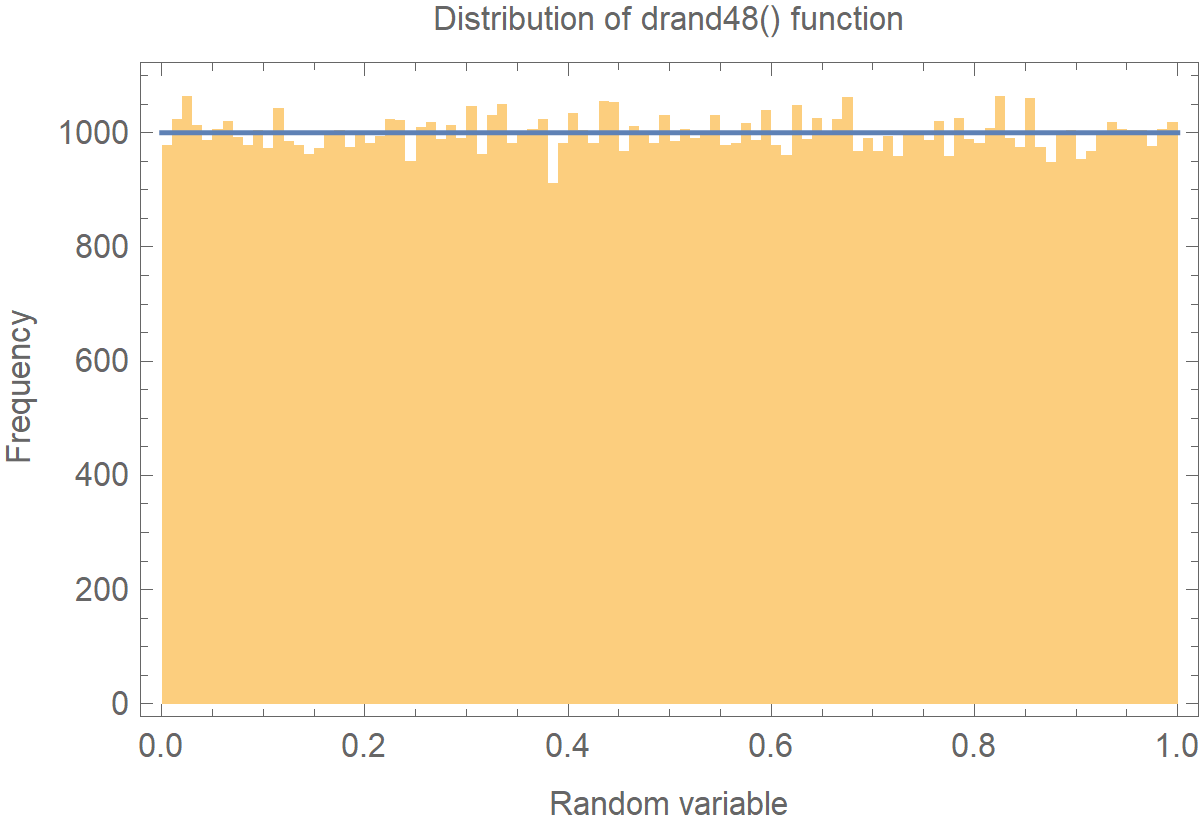
\includegraphics[width=4.4in]{homework7/uniform_dist.png}
    \caption{100-bin histogram (in gold) with 100 bins of 100,000 random numbers generated using \texttt{C}'s \texttt{drand48()} function. As expected, this conforms relatively closely to a uniform distribution of floating point numbers between 0 and 1, the PDF of which is shown in blue.}
    \label{fig:drand48}
\end{figure}

\begin{figure}[H]
    \centering
    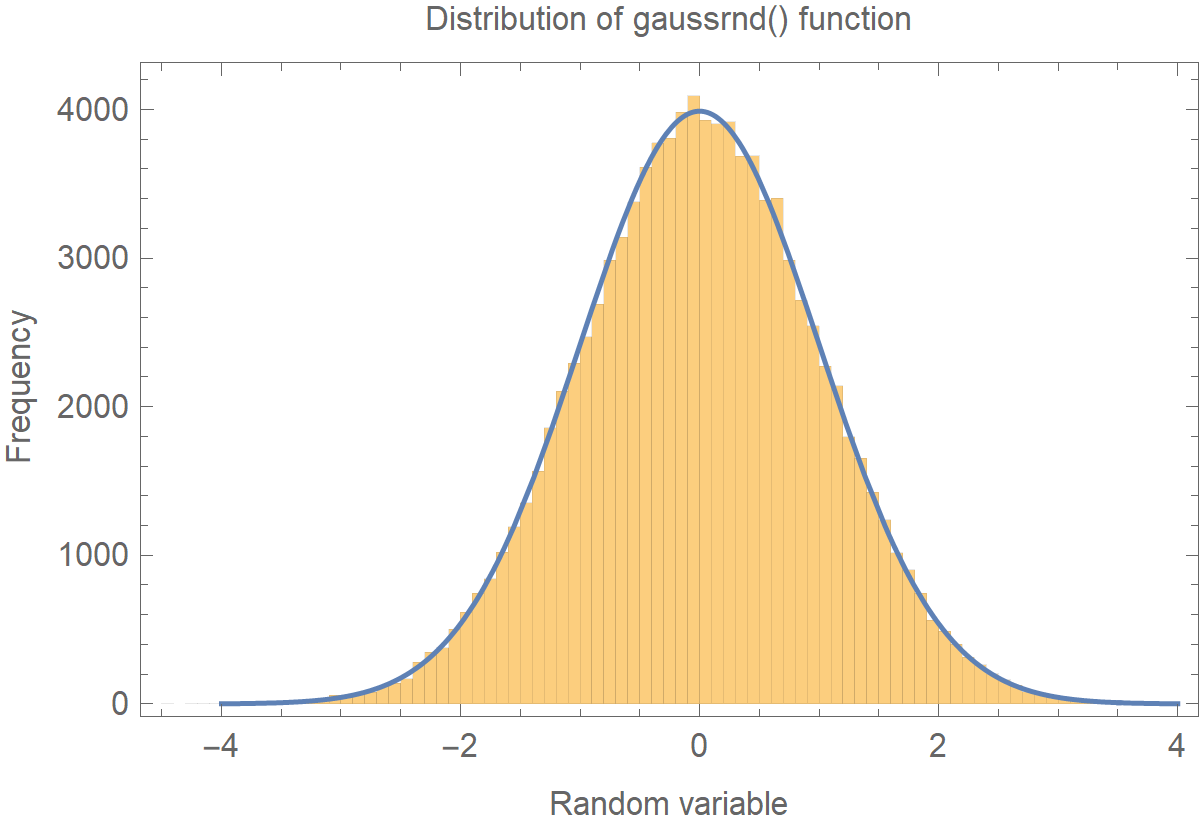
\includegraphics[width=4.4in]{homework7/normal_dist.png}
    \caption{100-bin histogram (in gold) of 100,000 random numbers generated using our \texttt{gaussrnd()} function. As expected, this conforms quite closely to a normal distribution with $\mu=1$ and $\sigma=1$, the PDF of which is shown in blue.}
    \label{fig:gaussrnd}
\end{figure}

\newpage

\bigskip
\noindent{\bf Question 2}
\medskip

\begin{figure}[H]
    \centering
    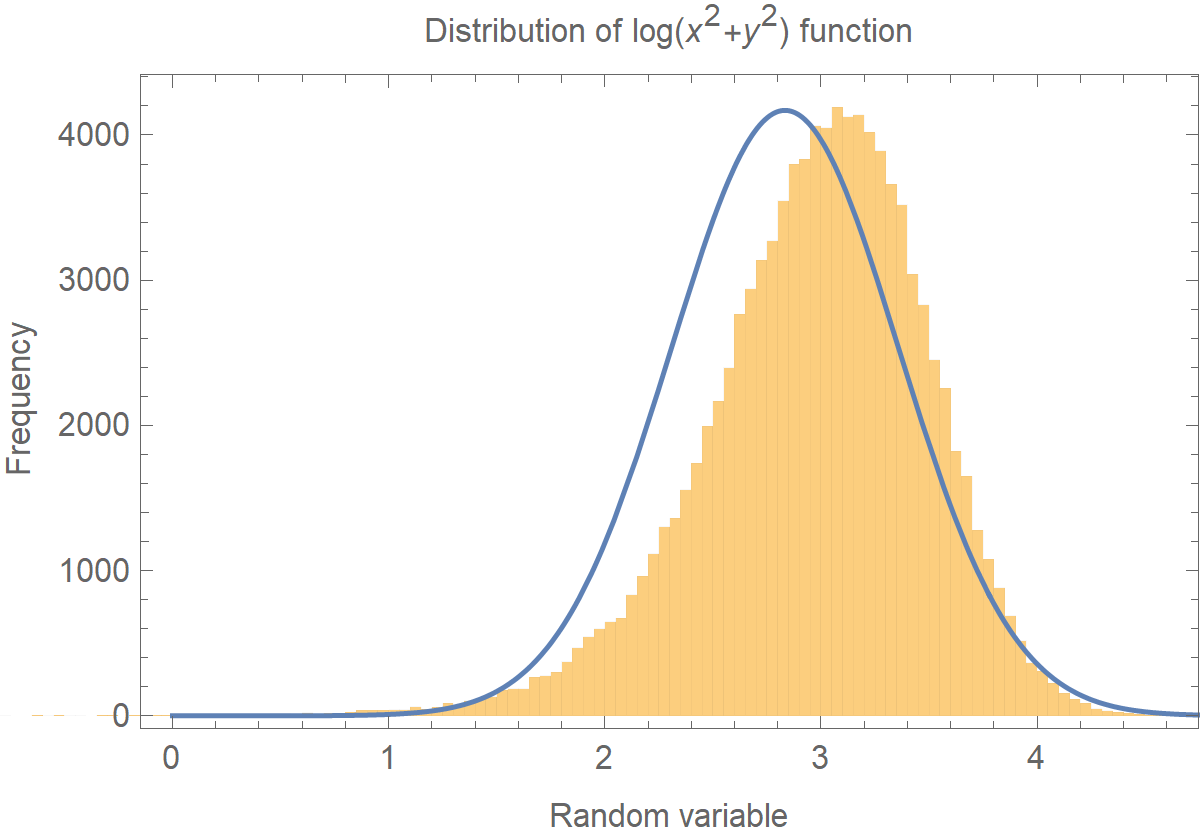
\includegraphics[width=4.4in]{homework7/log_dist.png}
    \caption{100-bin histogram (in gold) of 100,000 randomly generated numbers from the distribution $\log(x^2+y^2)$, where $x$ and $y$ are each uniformly-distributed variables with $\bar{x}=1$, $\bar{y}=4$, $\sigma_x=2$, and $\sigma_y=1$. The PDF of a normal distribution with $\mu=\log(1^2+4^2)=\log(17)$ and $\displaystyle \sigma^2=\left(\left.\frac{\partial f}{\partial x}\right|_{\bar{x},\bar{y}}\right)^2\sigma_x^2 + \left(\left.\frac{\partial f}{\partial y}\right|_{\bar{x},\bar{y}}\right)^2\sigma_y^2 = \frac{16\bar{x}^2}{(\bar{x}^2+\bar{y}^2)^2}+\frac{4\bar{y}^2}{(\bar{x}^2+\bar{y}^2)^2}=\frac{80}{289}$. This PDF is in less agreement with the distribution than in the previous problem because the logarithm throws off the normality of the selection. Although $x$ and $y$ are each normally distributed, taking the logarithm of the sum of their squares creates a sample of numbers that is not normal, so trying to ascribe a Gaussian function of $\mu$ and $\sigma$ in this way is not appropriate.}
    \label{fig:logx2y2}
\end{figure}

\newpage

\bigskip
\noindent{\bf Question 3}
\medskip

\begin{figure}[H]
    \centering
    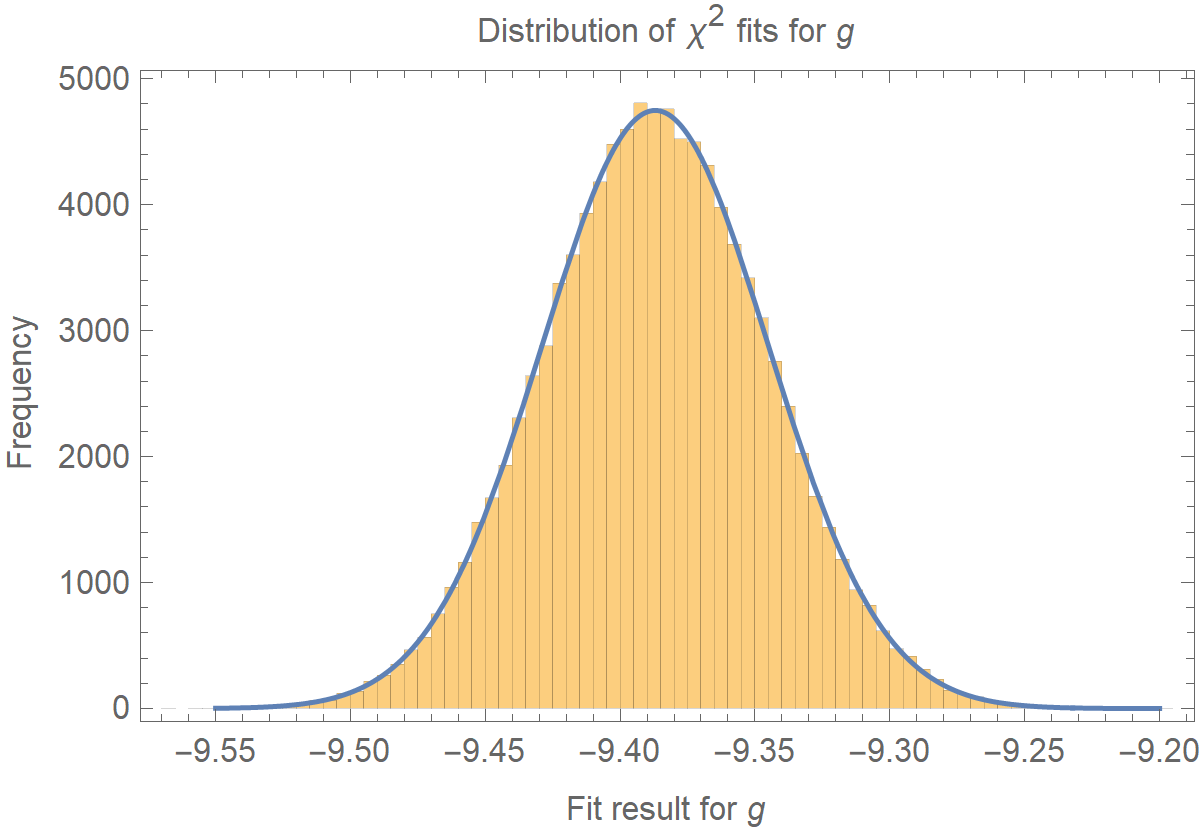
\includegraphics[width=4.5in]{homework7/g_hist.png}
    \caption{100-bin histogram (in gold) of the $\chi^2$ fit results for $g$ (the acceleration due to gravity) over 100,000 bootstrapped trials. The average result was $\bar{g}\cong-9.387$, with a standard deviation of $\sigma_g\cong0.042$ (the corresponding Gaussian PDF is shown in blue). Thus our routine has produced a result of $g=-9.387\pm0.042$, which interestingly does \emph{not} overlap with the accepted value of approximately $-9.81\text{ m/s}^2$.}
    \label{fig:g}
\end{figure}

\bigskip
\noindent{\bf Question 4}
\medskip

\noindent{\underline{Task 1:}}
\begin{figure}[H]
    \centering
    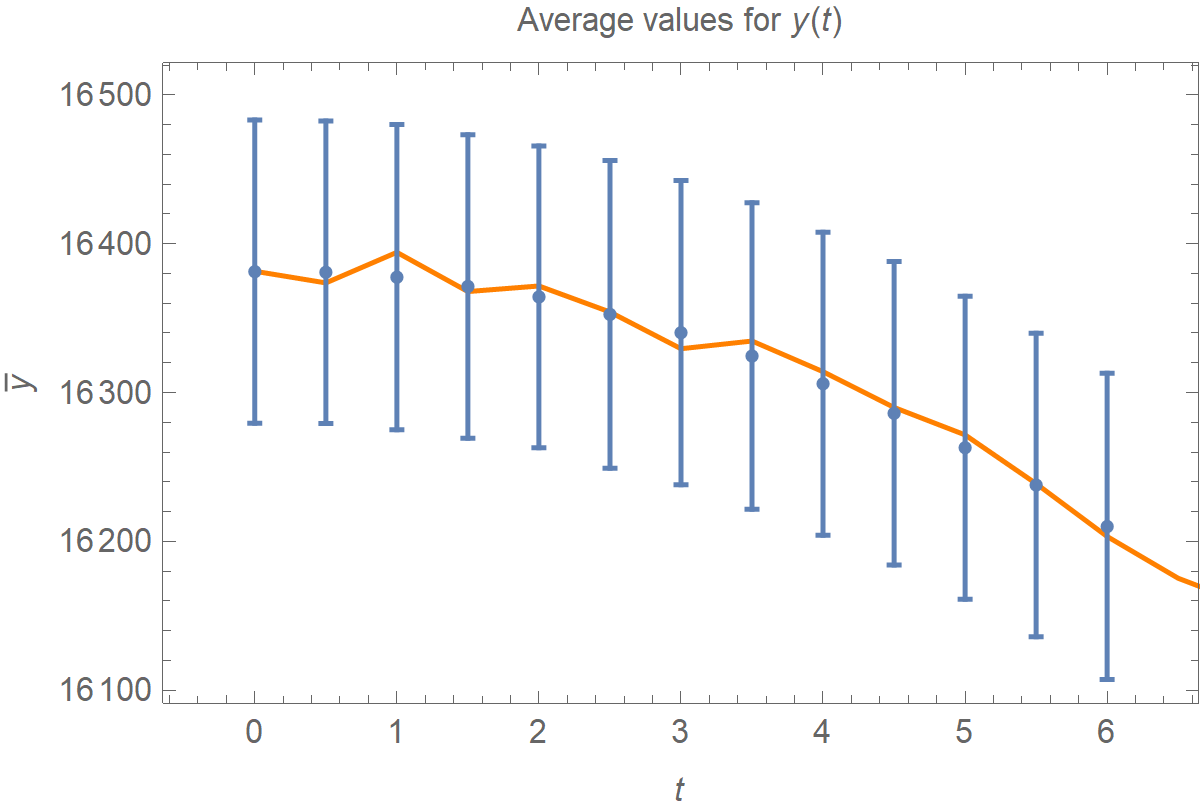
\includegraphics[width=4.5in]{homework7/yt_plot.png}
    \caption{Plot of average values from \texttt{bootstrap.dat} of $y(t)$ and their error for each time point $t$ (blue). As expected, this is quite similar to the trajectory in the first 6 seconds of \texttt{cannonball.dat}, which is plotted (without its error) in orange.}
    \label{fig:task1}
\end{figure}

\noindent{\underline{Task 2:}}
\begin{figure}[H]
    \centering
    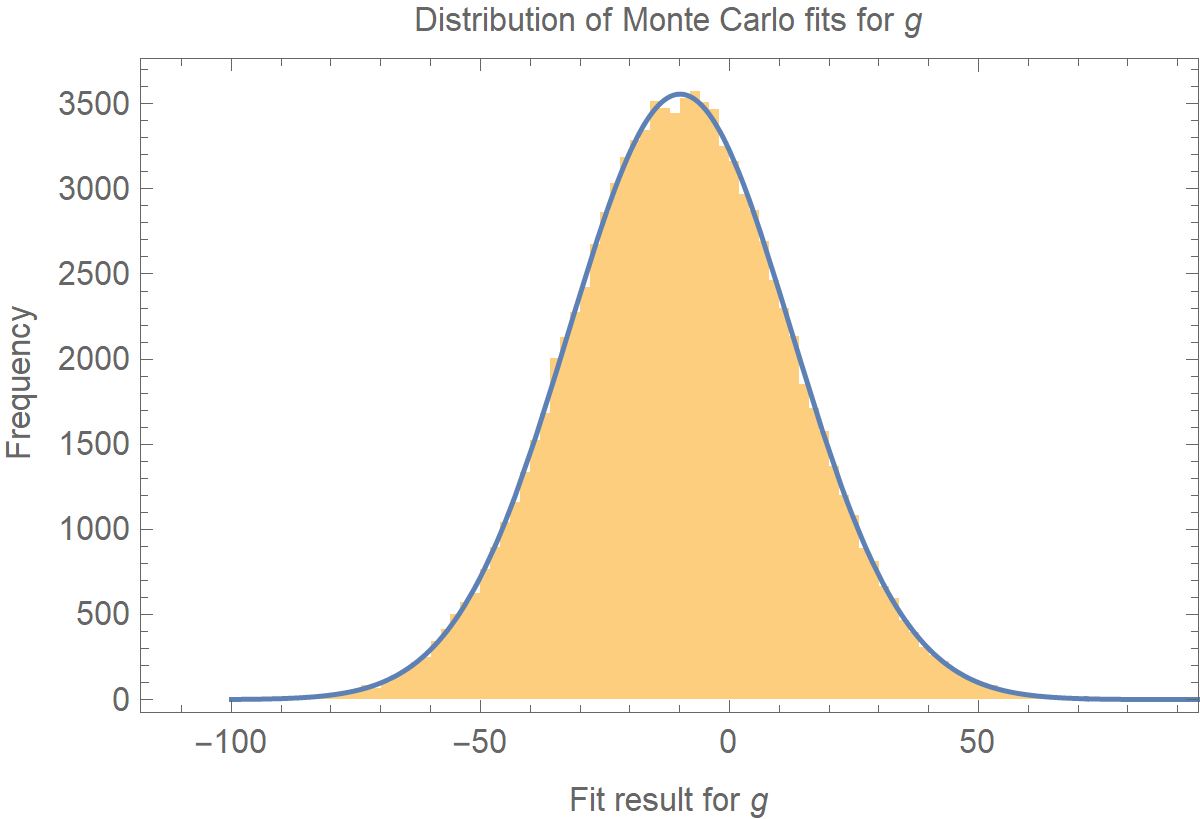
\includegraphics[width=4.5in]{homework7/task2hist.png}
    \caption{100-bin histogram (in gold) of Monte Carlo fit results for $g$, with a corresponding Gaussian PDF plotted over it in blue. This computation produced a result of $g=-9.925\pm22.428$, which is closer to the actual value of $g$ (and overlaps), but has a much higher uncertainty due to the large errors on the bootstrap data, as seen in Fig.~\ref{fig:task1}.}
    \label{fig:task2}
\end{figure}

\noindent{\underline{Task 3:}}
\begin{figure}[H]
    \centering
    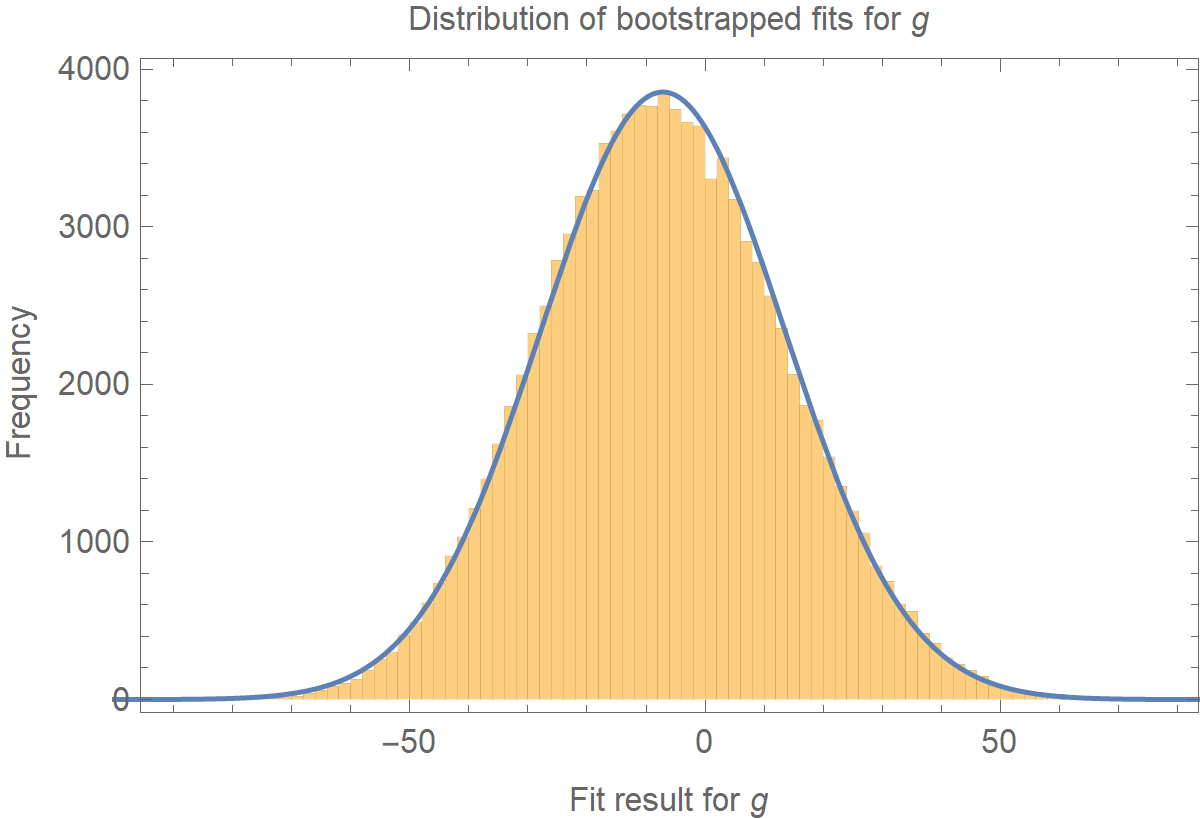
\includegraphics[width=4.5in]{homework7/task3hist.png}
    \caption{100-bin histogram (in gold) of bootstrap fit results for $g$, with a corresponding Gaussian PDF plotted over it in blue. This computation produced a result of $g=-7.16\pm20.69$. Although this technically overlaps with the correct value of $g$ due to its large error margin, this result is the least accurate nominal value yet. Again, this can be attributed to the large errors on the data itself. No fitting method or algorithm---no matter how clever---can overcome noisy or error-prone data.}
    \label{fig:task3}
\end{figure}

Another possible reason for the large fit uncertainties in the last two cases is the fact that there are, in some sense, only 12 data points, so the resampling process has a much higher capacity to produce vastly different coefficient fit results than when there are 117 (as in the original \texttt{cannonball.dat}).

\section{Conclusions}

Although a bit tricky on the coding side, I found this assignment to be a nice look into these techniques that are so common in scientific data analysis. The first few problems were a good conceptual introduction to the kind of thinking necessary to complete the more advanced ones.

I do wonder if there are more advanced methods one can employ that are more effective at dealing with large errors in datasets, and would be interested to learn more about this.


\end{document}
